\documentclass[12pt, letterpaper]{article}
\usepackage{setspace}
\usepackage{subcaption}
\usepackage[font={small,it}]{caption}\usepackage{graphicx}
\usepackage{array}
\usepackage{longtable}
\usepackage{quotes}
\usepackage{amsmath}
\usepackage{hyperref}
\usepackage[skip=10pt plus1pt, indent=40pt]{parskip}

% set reference files
\usepackage{biblatex}
\addbibresource{references.bib}

% set margins
\usepackage{geometry}
\geometry{margin=1in}

% Remove paragraph indentation
\setlength{\parindent}{0pt}


\graphicspath{{./figs/}{c:/Users/Zayan/Documents/code/personal_repos/neural_nets/ECE_8770/project_2/results}}
\onehalfspacing

\begin{document}

\begin{titlepage}
    \begin{center}

        \vspace*{1cm}

        \Large
        \textbf{ECE 8870 Project 2}

        \vspace{0.5cm}
        \textbf{Qazi Zarif Ul Islam}

        Pawprint: qzic2d

        \large

        \vspace{0.8cm}
        % \includegraphics[width=0.4\textwidth]{figs/Screenshot 2023-09-28 011032.png}

        University of Missouri-columbia \\
        04/21/2024
        
    \end{center}
\end{titlepage}
\tableofcontents

\section{Technical Description}

In this project, an RNN and an LSTM were implemented using pytorch.
The broader goal of this project was to understand the working principles of
RNNs and LSTMs and gain a comparative understanding of the two neural network
architectures. 

In the following sections, first the basic components of an RNN and an LSTM 
are introduced as well as an explanation of how backpropagation occurs in an 
RNN. This explanation will be more qualitative than mathematically rigorous. 
A more extensive treatment of backpropagation in RNNs can be found in ---. After that, the experiments and results shall be demonstrated and discussed before
a final conclustion section that talks about what more can be done to understand
RNNs and LSTMs and the deficiencies of this project.

The code is available at : \url{https://github.com/Murdock135/neural-nets-at-mizzou/tree/main/ECE_8770/project_2}

\subsection{Recurrent Neural Networks}

Recurrent Neural Networks are neural neural networks that store the 
hidden layer's output at the current time step so that it can influence
the output of the hidden layer at the next time step. Qualitatively,
this is commonly thought of as information being passed to the next time
step. Figure \ref{fig: rnns v1} shows this in two forms. On the left the 
rnn is said to be in "rolled"(in time) form whereas on the right is is said to be 
in "unrolled"(in time) form. The figure tells us that the rnn can be seen as a "feedback"
network of sorts where the output of the hidden layer $h_t$ is passed back to the hidden layer.
The left picture fails to capture that $h_t$ is passed to the next time step. The unrolled 
version captures this well. On the other hand, the rolled version captures a very crucial 
fact; that throughout the hidden layers at different time steps, \textit{there is only 
one weight matrix}, shared throughout the entire RNN at all time steps. Figure \ref{fig: rnns v2S} explicitly
illustrates this.

\begin{figure}[htpb]
    \centering
    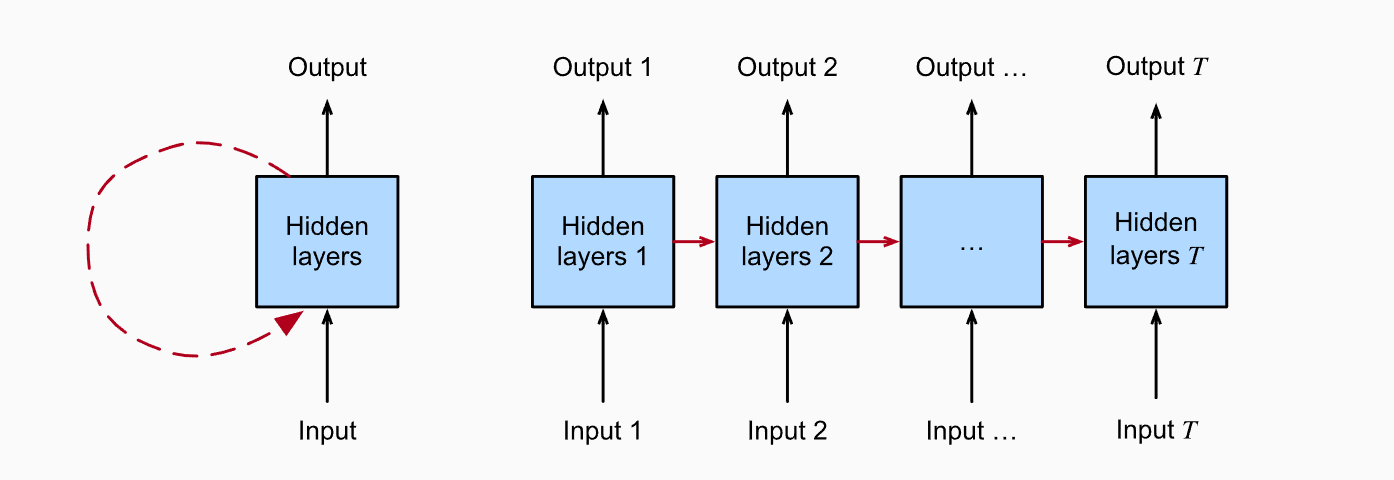
\includegraphics[width=0.8\textwidth]{d2l_ai_rnn_v1.png}
    \caption{\cite{zhang2023dive}: On the left recurrent connections are depicted via cyclic edges. 
    On the right, we unfold the RNN over time steps. Here, recurrent edges span 
    adjacent time steps, while conventional connections are computed synchronously}
    \label{fig: rnns v1}
\end{figure}

The shaded blue boxes are each a Multi-layer perceptron. The only caveat here is that in addition to the
inputs of the "current time step" $x_t$, it also recieves \textit{as} input, the weighted outputs of 
the previous hidden layer $h_{t-1}$. Thus, the input to the current hidden layer is expressed as a 
concatenation $[h_{t-1};\;x_t]$. Thus the equations defining the RNN are,

\begin{align}
    h_t = \phi(W_{hh} h_{t-1} + W_{xh} x_t + b_h)
    \label{eqn: h_t rnn}
\end{align}

\begin{equation}
    o_t = W_o h_t + b_o
    \label{eqn: o_t rnn}
\end{equation}

Where in equation \ref{eqn: h_t rnn}, $W_{hh}$ indicates \textbf{the weights going from the hidden layer at the previous time step to the 
hidden layer at the current time step}, $W_{xh}$ indicates \textbf{the weights going from the current 
inputs to the current hidden layer.} In equation \ref{eqn: o_t rnn} $W_o$ indicates \textbf{the weights going from
the hidden layer at the current time step to the output layer of the current time step.}

With these equations, the learning rule the RNN can be derived for any optimization algorithm e.g.
stochastic gradient descent, adaptive momentum, RMS prop, etc. The algorithms won't be discussed in 
this report but the gradients of the error wrt the learnable parameters are mentioned
in the next section, \textbf{backpropagation through time}.

\subsubsection{Backpropagation through time (Backpropagation for RNNs)}

\begin{figure}[htpb]
    \centering
    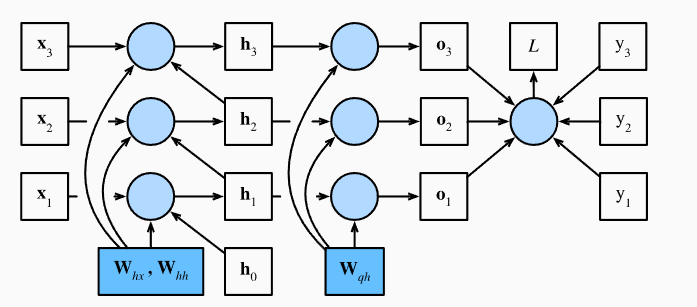
\includegraphics[width=0.8\textwidth]{d2l_ai_rnn_v2.png}
    \caption{\cite{zhang2023dive}: Computational graph showing dependencies for an RNN model 
    with three time steps. Boxes represent variables (not shaded) or parameters (shaded) and circles 
    represent operators.}
    \label{fig: rnns v2}
\end{figure}


For an RNN, the total loss is expressed as,

\begin{equation}
    \hat{L} = \frac{1}{T} \sum_{t=1}^{T} \ell(y_t, d_t) = \frac{1}{T} (l_1 + l_2 + ... + l_t ... + l_T)
    \label{eqn: total loss rnn}
\end{equation}

Where the small $l_t$'s indicate loss at a particular time step. The gradients of this total loss with respect
to the learnable parameters are, 

\begin{align}
    \frac{\partial l_t}{\partial w_h} &= \frac{\partial l_t}{\partial o_t}\frac{\partial o_t}{\partial h_t}\frac{\partial h_t}{\partial w_h} \label{eqn: rnn lt wrt w_h}\\
    \frac{\partial h_t}{\partial w_h} &= \frac{\partial h_t}{\partial w_h} + \sum_{i=1}^{t-1}\prod_{j-1=i}^{t} (\frac{\partial h_j}{\partial h_{j-1}}) \frac{\partial h_i}{\partial w_h}\label{eqn: rnn h_t wrt w_h}\\
    \frac{\partial L}{\partial W_{oh}} &= \sum_{t}^{T} \frac{\partial L}{\partial o_t} h_t \\
    \frac{\partial L}{\partial W_{hx}} &= \sum_{t}^{T} \frac{\partial L}{\partial h_t} x_t \\
    \frac{\partial L}{\partial w_h} &= \sum_{t}^T \frac{\partial l_t}{\partial o_t}\frac{\partial o_t}{\partial h_t}\frac{\partial h_t}{\partial w_h} \label{eqn: rnn total loss wrt w_h}
\end{align}

Where $w_h = [W_{hx};\; W_{hh}]$ is the concatenated weight matrix, 
$W_{oh}$ is the weight matrix from the hidden layer to the output layer, 
$W_{hx}$ is the weight matrix from the input layer to the hidden layer.

Observe equation \ref{eqn: rnn h_t wrt w_h}. Any gradient based algorithm would compute
this gradient and when it does, it has to recursively calculate the change of 
$h_j$ wrt $h_{j-1}$ and if the sequence is long, this product term will 
either be very large (if each gradient term $>1$) or be miniscule (if each gradient 
term $<1$). These two situations are called the \textit{exploding gradient} and 
the \textit{diminishing or vanishing gradient} problems, respectively. To solve
this issue, several techniques are used to truncate this product. \cite{zhang2023dive}
mentions two such techniques; \textit{(1) Regular truncation} and \textit{(2) Randomized
truncation.} The equations won't be derived in this report but an illustration of 
the three techniques is presented in fig \ref{fig: truncated_bptt}. In regular 
truncated BPTT, the sum is truncated after $\tau$ steps whereas in 
randomized BPTT, the initial sequences are split up into sub-sequences 
of "random" length (here, the length of the subsequences are cast as random
variables). \cite{tallec2017unbiasing}

\begin{figure}[htpb]
    \centering
    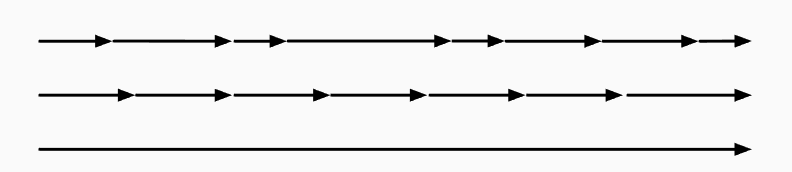
\includegraphics[width=0.8\textwidth]{techniques for truncated bptt.png}
    \caption{Comparing strategies for computing gradients in RNNs. From top to bottom: randomized truncation, regular truncation, and full computation.}
    \label{fig: truncated_bptt}
\end{figure}

\subsection{Long Short Term Memory nets (LSTMs)}

\begin{figure}[htpb]
    \centering
    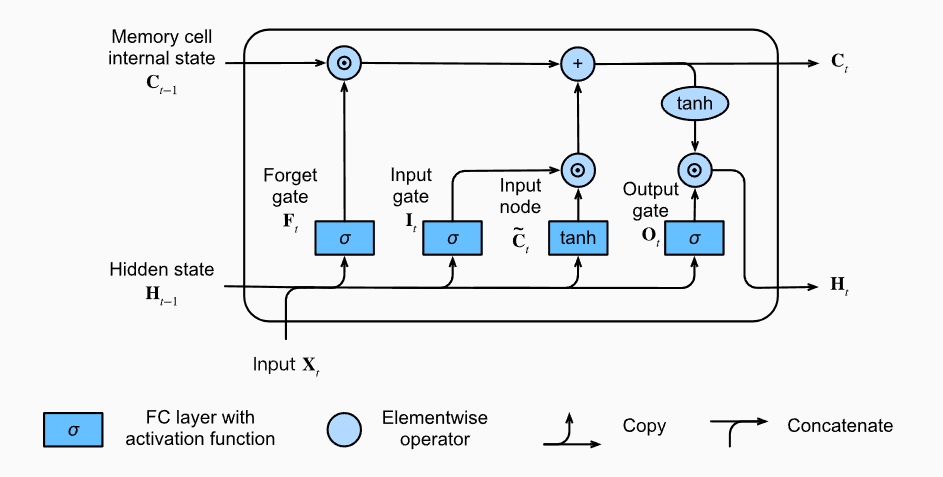
\includegraphics[width=0.8\textwidth]{lstms v1.png}
    \caption{lstms}
    \label{fig: lstms}
\end{figure}

LSTMs resemble RNNs but each recurrent node is replaced by a memory cell, which is not composed
of just traditional neural units that compute a function of the weighted inputs. It is rather
a combination of different kinds of operators (here I'm calling a neuron an operator) that
allow controlling \textbf{the degree to which the previous hidden state $H_{t-1}$, the current 
hidden state $H_t$ and current input $X_t$ influences the current outputs}. Each cell will 
output 2 quantities; (1) The current cell state $C_t$ and (2) The current hidden state $H_t$.

While RNNs have \textit{long term memory} in the form of shared weights $W_{hh}$, LSTMs
have both long term and \textit{short term memory} where the very act of controlling the 
aforementioned quantities is the short term memory aspect.\cite{zhang2023dive}

The term `gate' is often used to describe the operators in an LSTMs, probably owing 
to their ability to control a particular quantity's importance in computing the 
current hidden state and cell state. This gating functionality will be more apparent
from the equations that describe fig \ref{fig: lstms}. I'll introduce the equations 
in a backwards fashion, with the outputs first and inputs last.

\begin{align}
    C_t &= F_t \odot C_{t-1} + I_t \odot \tilde{C_t}\\
    H_t &= O_t \odot tanh(C_t)
\end{align}

where $\odot$ is the element wise product operator, $I_t$ is the output of the \textbf{Input gate}, 
$F_t$ is the output of the \textbf{forget gate}, $O_t$ is the output of the \textbf{output gate} and 
$\tilde{C_t}$ is the output of the \textbf{Input Node}. These are given by,

\begin{align}
    I_t &= \sigma(X_t W_{xi} + H_{t-1} W_{hi} b_i)\\
    F_t &= \sigma(X_t W_{xf} + H_{t-1} W_{hf} b_f)\\
    O_t &= \sigma(X_t W_{xo} + H_{t-1} W_{ho} b_o)\\
    \tilde{C_t} &= tanh(X_t W_{xc} + H_{t-1} W_{hc} + b_c)
\end{align}



\subsection{RNN/LSTM configurations}

There are 4 common setting that an RNN or LSTM can be used. Figure \ref{fig: RNN/LSTM configs}
illustrates these settings. The first is a one to one setting, where one input predicts one output. 
The second is a one to many setting where one input predicts multiple outputs. For example, if we let 
the model use the stock price of one day and ask it to predict the stock price of 3 days in the future,
that is a one to many setting. The final setting, many to many, as 2 versions; version 1 is where 
multiple inputs \textit{in the past} predict multiple things about the future and version 2 is 
a bit like the one to one setting, the only difference being that several one-to-one configurations
have been chained together. 

\begin{figure}[htpb]
    \centering
    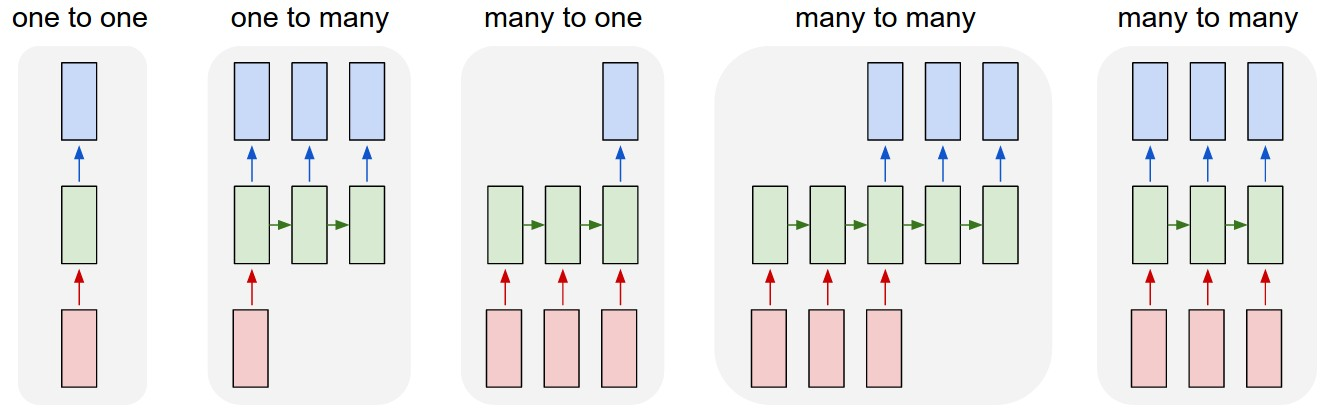
\includegraphics[width=0.8\textwidth]{rnn configurations.jpeg}
    \caption{From the left, the first picture is the one-to-one configuration, 
    the second is the one-to-many configuration, third is version-1 of the many-to-many
    configuration and the fourth is version-2 of the many-to-many configuration.}
    \label{fig: RNN/LSTM configs}
\end{figure}

\section{Experiments and Results}

To study RNNs and LSTMs in practice, experiments were run where the the models are used to forecast the closing price of stock prices of microsoft inc.
The following parameters were varied.

\begin{enumerate}
    \item Model type; whether it is an RNN or LSTM.
    \item The sequence length (varied between sequence lengths of 3, 7, 50 and 100).
    \item The `future strategy'; whether it predicts sequentially (version-2 of many-to-many) or many to one.
    \item The optimizer (Adam and SGD). Note that when the Adam optimizer is used, the model 
    is trained for 10 epochs, when SGD is used, the model is trained for 100 epochs.
\end{enumerate}

All possible combinations were experimented with but only the most insightful results will be shown here
for the sake of brevity. Note that the Mean Squared Error (MSE) measure was 
used as the loss for all models. Furthermore, A hidden layer 
size of 512 units for both types of models (rnn and lstm).

\subsection{Training details}

The following experiments were run on an NVIDIA CUDA RTX 3050 laptop GPU. The
machine has a total memory of 16 GigaBytes. Each experiment was run for 100 epochs.
The dataset was partitioned into batches of 32 samples. 

\textbf{Dataset}

The model was trained on stock price dataset and can be found here 
https://www.kaggle.com/datasets/vijayvvenkitesh/microsoft-stock-time-series-analysis.
Specifically, it was trained on the `closing price' of the stock price. The stock 
price pertains to microsoft inc. 80\% of the data was used as training data and 
cross validation wasn't used.

\subsection{Results}

\begin{itemize}
    \item From figure \ref{fig: SGD-RNN forecast results as sequence length is varied in a sequential setting}
    and figure \ref{fig: SGD-LSTM forecast results as sequence length is varied in a sequential setting}
    the first key observation we can make is that the \textbf{RNN's predictions
    vary considerably more from one time step to the next than that of the 
    LSTMs} in both sequential\footnote{Here I'm using the terms 'many To
    many' and 'sequential' interchangabley.} and many to many setting. 

    \item In a many to one setting, the predictions of both RNN and LSTM are less zigzaggy and more stable in a sense (fig
    \ref{fig: SGD-RNN forecast results as sequence length is varied in a many-to-one setting}).
    It seems as though in a many to many setting, where only the previous
    time step predicts the next, the models are less sure and has to change their 
    predictions drastically once it recieves a latter input in the sequence. Furthermore,
    the zigzaggy effect seems to increase with increase of sequence length for both 
    types of models. This is possibly due to large error gradients as sequence length increases.
    . After all, the larger the sequence length the larger the gradient computed in equation \ref{eqn: rnn h_t wrt w_h}.
    
    \item Comparing fig \ref{fig: SGD-LSTM forecast results as sequence length is varied in a sequential setting}
    and fig \ref{fig: Adam-LSTM forecast results as sequence length is varied in a sequential setting}
    , it seems that the LSTM fails to learn or update its weights optimally
    when it is optimized via SGD.

    \item If we compare figure \ref{fig: Adam-RNN forecast results as sequence length is varied in a sequential setting} 
    and fig \ref{fig: Adam-LSTM forecast results as sequence length is varied in a sequential setting}, both models 
    again show an increase of the zigzaggy effect as sequence length increases but what's more interesting is 
    that the RNN shows better results, confirmed by the figure \ref{Validation loss of all models after training} 
    where the loss-on-validation-set of the model has been tabled. Observe for a sequence length of 50, many-to-many setting and under Adam optimization, 
    that the RNN incurs a loss of 0.0005 while that of LSTM is 0.001 
    
    \item Overall, all models predict near true values across time when optimized via Adam.
\end{itemize}


% SGD RESULTS
% SGD-RNN forecast results as sequence length is varied in a sequential setting
\begin{figure}[htpb]
    \centering
    \begin{subfigure}[b]{0.3\textwidth}
        \includegraphics[width=\textwidth]{c:/Users/Zayan/Documents/code/personal_repos/neural_nets/ECE_8770/project_2/results/2024-04-24_17-34-00__rnn_3_sequential_sgd_[0.001]_forecast.jpg}
    \end{subfigure}
    \begin{subfigure}[b]{0.3\textwidth}
        \includegraphics[width=\textwidth]{c:/Users/Zayan/Documents/code/personal_repos/neural_nets/ECE_8770/project_2/results/2024-04-24_17-34-35__rnn_7_sequential_sgd_[0.001]_forecast.jpg}
    \end{subfigure}
    \begin{subfigure}[b]{0.3\textwidth}
        \includegraphics[width=\textwidth]{c:/Users/Zayan/Documents/code/personal_repos/neural_nets/ECE_8770/project_2/results/2024-04-24_17-35-30__rnn_50_sequential_sgd_[0.001]_forecast.jpg}
    \end{subfigure}
    \caption{RNN(optimized by SGD) forecast results as sequence length is varied in a sequential setting}
    \label{fig: SGD-RNN forecast results as sequence length is varied in a sequential setting}
\end{figure}

% SGD-LSTM forecast results as sequence length is varied in a sequential setting
\begin{figure}[htpb]
    \centering
    \begin{subfigure}[b]{0.3\textwidth}
        \includegraphics[width=\textwidth]{c:/Users/Zayan/Documents/code/personal_repos/neural_nets/ECE_8770/project_2/results/2024-04-24_17-37-51__lstm_3_sequential_sgd_[0.001]_forecast.jpg}
    \end{subfigure}
    \begin{subfigure}[b]{0.3\textwidth}
        \includegraphics[width=\textwidth]{c:/Users/Zayan/Documents/code/personal_repos/neural_nets/ECE_8770/project_2/results/2024-04-24_17-38-24__lstm_7_sequential_sgd_[0.001]_forecast.jpg}
    \end{subfigure}
    \begin{subfigure}[b]{0.3\textwidth}
        \includegraphics[width=\textwidth]{c:/Users/Zayan/Documents/code/personal_repos/neural_nets/ECE_8770/project_2/results/2024-04-24_17-39-23__lstm_50_sequential_sgd_[0.001]_forecast.jpg}
    \end{subfigure}
    \caption{LSTM(optimized by SGD) forecast results as sequence length is varied in a sequential setting}
    \label{fig: SGD-LSTM forecast results as sequence length is varied in a sequential setting}
\end{figure}

% SGD-RNN forecast results as sequence length is varied in a many to one setting
\begin{figure}[htpb]
    \centering
    \begin{subfigure}[b]{0.3\textwidth}
        \includegraphics[width=\textwidth]{c:/Users/Zayan/Documents/code/personal_repos/neural_nets/ECE_8770/project_2/results/2024-04-24_17-34-15__rnn_3_many_to_one_sgd_[0.001]_forecast.jpg}
    \end{subfigure}
    \begin{subfigure}[b]{0.3\textwidth}
        \includegraphics[width=\textwidth]{c:/Users/Zayan/Documents/code/personal_repos/neural_nets/ECE_8770/project_2/results/2024-04-24_17-34-51__rnn_7_many_to_one_sgd_[0.001]_forecast.jpg}
    \end{subfigure}
    \begin{subfigure}[b]{0.3\textwidth}
        \includegraphics[width=\textwidth]{c:/Users/Zayan/Documents/code/personal_repos/neural_nets/ECE_8770/project_2/results/2024-04-24_17-35-57__rnn_50_many_to_one_sgd_[0.001]_forecast.jpg}
    \end{subfigure}
    \caption{RNN(optimized by SGD) forecast results as sequence length is varied in a many to one setting}
    \label{fig: SGD-RNN forecast results as sequence length is varied in a many-to-one setting}
\end{figure}

% SGD-LSTM forecast results as sequence length is varied in a many to one setting
\begin{figure}[htpb]
    \centering
    \begin{subfigure}[b]{0.3\textwidth}
        \includegraphics[width=\textwidth]{c:/Users/Zayan/Documents/code/personal_repos/neural_nets/ECE_8770/project_2/results/2024-04-24_17-38-05__lstm_3_many_to_one_sgd_[0.001]_forecast.jpg}
    \end{subfigure}
    \begin{subfigure}[b]{0.3\textwidth}
        \includegraphics[width=\textwidth]{c:/Users/Zayan/Documents/code/personal_repos/neural_nets/ECE_8770/project_2/results/2024-04-24_17-38-39__lstm_7_many_to_one_sgd_[0.001]_forecast.jpg}
    \end{subfigure}
    \begin{subfigure}[b]{0.3\textwidth}
        \includegraphics[width=\textwidth]{c:/Users/Zayan/Documents/code/personal_repos/neural_nets/ECE_8770/project_2/results/2024-04-24_17-39-57__lstm_50_many_to_one_sgd_[0.001]_forecast.jpg}
    \end{subfigure}
    \caption{LSTM(optimized by SGD) forecast results as sequence length is varied in a many to one setting}
    \label{fig: SGD-LSTM forecast results as sequence length is varied in a many-to-one setting}
\end{figure}

% ADAM RESULTS
% Adam-RNN forecast results as sequence length is varied in a sequential setting
\begin{figure}[htpb]
    \centering
    \begin{subfigure}[b]{0.3\textwidth}
        \includegraphics[width=\textwidth]{c:/Users/Zayan/Documents/code/personal_repos/neural_nets/ECE_8770/project_2/results/2024-04-24_17-33-44__rnn_3_sequential_adam_[0.001]_forecast.jpg}
    \end{subfigure}
    \begin{subfigure}[b]{0.3\textwidth}
        \includegraphics[width=\textwidth]{c:/Users/Zayan/Documents/code/personal_repos/neural_nets/ECE_8770/project_2/results/2024-04-24_17-34-18__rnn_7_sequential_adam_[0.001]_forecast.jpg}
    \end{subfigure}
    \begin{subfigure}[b]{0.3\textwidth}
        \includegraphics[width=\textwidth]{c:/Users/Zayan/Documents/code/personal_repos/neural_nets/ECE_8770/project_2/results/2024-04-24_17-34-57__rnn_50_sequential_adam_[0.001]_forecast.jpg}
    \end{subfigure}
    \caption{RNN(optimized by Adam) forecast results as sequence length is varied in a sequential setting}
    \label{fig: Adam-RNN forecast results as sequence length is varied in a sequential setting}
\end{figure}

% Adam-RNN forecast results as sequence length is varied in a many to one setting
\begin{figure}[htpb]
    \centering
    \begin{subfigure}[b]{0.3\textwidth}
        \includegraphics[width=\textwidth]{c:/Users/Zayan/Documents/code/personal_repos/neural_nets/ECE_8770/project_2/results/2024-04-24_17-33-46__rnn_3_many_to_one_adam_[0.001]_forecast.jpg}
    \end{subfigure}
    \begin{subfigure}[b]{0.3\textwidth}
        \includegraphics[width=\textwidth]{c:/Users/Zayan/Documents/code/personal_repos/neural_nets/ECE_8770/project_2/results/2024-04-24_17-34-20__rnn_7_many_to_one_adam_[0.001]_forecast.jpg}
    \end{subfigure}
    \begin{subfigure}[b]{0.3\textwidth}
        \includegraphics[width=\textwidth]{c:/Users/Zayan/Documents/code/personal_repos/neural_nets/ECE_8770/project_2/results/2024-04-24_17-35-00__rnn_50_many_to_one_adam_[0.001]_forecast.jpg}
    \end{subfigure}
    \caption{RNN(optimized by Adam) forecast results as sequence length is varied in a many to one setting}
    \label{fig: Adam-RNN forecast results as sequence length is varied in a many-to-one setting}
\end{figure}

% Adam-LSTM forecast results as sequence length is varied in a sequential setting
\begin{figure}[htpb]
    \centering
    \begin{subfigure}[b]{0.3\textwidth}
        \includegraphics[width=\textwidth]{c:/Users/Zayan/Documents/code/personal_repos/neural_nets/ECE_8770/project_2/results/2024-04-24_17-37-35__lstm_3_sequential_adam_[0.001]_forecast.jpg}
    \end{subfigure}
    \begin{subfigure}[b]{0.3\textwidth}
        \includegraphics[width=\textwidth]{c:/Users/Zayan/Documents/code/personal_repos/neural_nets/ECE_8770/project_2/results/2024-04-24_17-38-08__lstm_7_sequential_adam_[0.001]_forecast.jpg}
    \end{subfigure}
    \begin{subfigure}[b]{0.3\textwidth}
        \includegraphics[width=\textwidth]{c:/Users/Zayan/Documents/code/personal_repos/neural_nets/ECE_8770/project_2/results/2024-04-24_17-38-45__lstm_50_sequential_adam_[0.001]_forecast.jpg}
    \end{subfigure}
    \caption{LSTM(optimized by Adam) forecast results as sequence length is varied in a sequential setting}
    \label{fig: Adam-LSTM forecast results as sequence length is varied in a sequential setting}
\end{figure}

% Adam-LSTM forecast results as sequence length is varied in a many-to-one setting
\begin{figure}[htpb]
    \centering
    \begin{subfigure}[b]{0.3\textwidth}
        \includegraphics[width=\textwidth]{c:/Users/Zayan/Documents/code/personal_repos/neural_nets/ECE_8770/project_2/results/2024-04-24_17-37-37__lstm_3_many_to_one_adam_[0.001]_forecast.jpg}
    \end{subfigure}
    \begin{subfigure}[b]{0.3\textwidth}
        \includegraphics[width=\textwidth]{c:/Users/Zayan/Documents/code/personal_repos/neural_nets/ECE_8770/project_2/results/2024-04-24_17-38-10__lstm_7_many_to_one_adam_[0.001]_forecast.jpg}
    \end{subfigure}
    \begin{subfigure}[b]{0.3\textwidth}
        \includegraphics[width=\textwidth]{c:/Users/Zayan/Documents/code/personal_repos/neural_nets/ECE_8770/project_2/results/2024-04-24_17-38-49__lstm_50_many_to_one_adam_[0.001]_forecast.jpg}
    \end{subfigure}
    \caption{LSTM(optimized by Adam) forecast results as sequence length is varied in a many-to-one setting}
    \label{fig: Adam-LSTM forecast results as sequence length is varied in a many-to-one setting}
\end{figure}

\begin{figure}
    \centering
    \includegraphics[width=0.6\textwidth]{c:/Users/Zayan/Documents/code/personal_repos/neural_nets/ECE_8770/project_2/results/results_consolidated_pic.png}
    \caption{Validation loss of all models after training}
    \label{fig: table of results}
\end{figure}

\section{Conclusion}

RNNs and LSTMs are suitable for data where the samples can be imagined as 
sequentially progressing e.g. samples over time or samples where an aspect is 
sequentially dependent on another aspect that's in the past. For this project 
however, samples over time have been considered only. Meaning, a forecasting problem 
has been used. Both an RNN and an LSTM were used to forecast the stock price of a company.
The striking property of RNNs known as the exploding gradient (sometimes `vanishing') has 
been discovered in this practical setting. Furthermore, the effect of varying 
sequence lengths and varying settings have been observed. Whether a many-to-many 
or many-to-one setting is better for all problems is not known, as the results didn't
suggest a clear winner among the two. However, the `zigzaggy' effect that the increase 
of sequence length invokes has been seen as a recurrent occurance. 

For this project, the reason for choosing the dataset is seasonality. Since the 
stock price increases as the years progress, it seemed like a good question to ask 
how well the RNNs and LSTMs can predict this increase. However, if datasets with no
seasonality or other properties are selected, perhaps other effects would come to light.
Thus, as a future work, I suggest using datasets with no seasonality and other properties 
to further study RNNs and LSTMs. 

\clearpage
\printbibliography

\appendix

\section{Proof of equation \ref{eqn: rnn h_t wrt w_h}}

The emprical loss of the neural network is,

\begin{equation}
    \hat{L} = \frac{1}{T} \sum_{t=1}^{T} \ell(y_t, d_t) = \frac{1}{T} (l_1 + l_2 + ... + l_t ... + l_T)
\end{equation}

For an RNN, the system is defined by,
\begin{align}
    h_{t} &= f (X_{t}, h_{t-1}) = \phi_{h}(W_{xh} \cdot X_{t} + W_{hh}\cdot h_{t-1} +b_{h}) \\
    \hat{o}_{t} &= f_{o}(h_{t}) = \phi_{o}(W_{hy}\cdot h_{t} + b_{y})
\end{align}

Let $w_h = [W_{xh}\;W_{hh}]^T$.

Thus,

\begin{equation}
    \frac{\partial \hat{L}}{\partial w_h} = \frac{1}{T} (\frac{\partial l_1}{\partial w_h} + \frac{\partial l_2}{\partial w_h} + ... + \frac{\partial l_t}{\partial w_h} ... + \frac{\partial l_T}{\partial w_h})
\end{equation}

Now the loss at a particular time instant t follows the chain rule of derivatives.

\begin{equation}
    \frac{\partial l_t}{\partial w_h} = \frac{\partial l_t}{\partial o_t}\frac{\partial o_t}{\partial h_t}\frac{\partial h_t}{\partial w_h}
    \label{eq: l_t}
\end{equation}

But $h_t$ is a function of $h_{t-1}$ and $w_h$ as well (besides $X_t$).
Furthermore, $h_{t-1}$ is again a function of $w_h$.
Thus, by the multivariable chain rule,

If $h_t = f_1(h_{t-1}, w_h), h_{t-1}= g_1(h_{t-2}, w_h), w_h = h_1(w_h)$ \footnote{(Note: $h_1$ (the function, \textit{not} the hidden state) is merely the identity
function. We've formulated it so just to be consistent with the
formulation of "case 1" in \cite{multivariate_chain_rule}. Eqn \ref{eq: h_t wrt wh} would still 
be valid even if we hadn't defined it as a separate function.} (Read as "The function $f_1$ takes 
$h_{t-1}$ and $w_h$ as input, $g_1$ takes $h_{t-2}$ and $w_h$ as input and $h_1$ takes $w_h$ as input.)

\begin{equation}
    \frac{\partial h_t}{\partial w_h} = \frac{\partial f_1}{\partial w_h} + \frac{\partial f_1}{\partial h_{t-1}}\frac{\partial h_{t-1}}{\partial w_h}
    \label{eq: h_t wrt wh}
\end{equation}

Similarly, if $h_{t-1} = f_2(h_{t-2}, w_h), h_{t-2}= g_2(h_{t-3}, w_h), w_h = h_2(w_h)$

\begin{equation}
    \frac{\partial h_{t-1}}{\partial w_h} = \frac{\partial f_2}{\partial w_h} + \frac{\partial f_2}{\partial h_{t-2}}\frac{\partial h_{t-2}}{\partial w_h}
    \label{eq: h_t-1 wrt wh}
\end{equation}

Similarly, if $h_{t-2} = f_3(h_{t-3}, w_h), h_{t-3}= g_3(h_{t-4}, w_h), w_h = h_3(w_h)$

\begin{equation}
    \frac{\partial h_{t-2}}{\partial w_h} = \frac{\partial f_3}{\partial w_h} + \frac{\partial f_3}{\partial h_{t-3}}\frac{\partial h_{t-3}}{\partial w_h}
    \label{eq: h_t-2 wrt wh}
\end{equation}

We can find similar expressions for time steps further back $h_{t-3}, h_{t-4}$ all the way to $h_1$.

Now, from equation \ref{eq: h_t wrt wh} and equation \ref{eq: h_t-1 wrt wh}, 

\begin{align}
    \frac{\partial h_t}{\partial w_h} &= \frac{\partial f_1}{\partial w_h} + \frac{\partial f_1}{\partial h_{t-1}}(\frac{\partial f_2}{\partial w_h} + \frac{\partial f_2}{\partial h_{t-2}}\frac{\partial h_{t-2}}{\partial w_h}) && (\text{we won't expand $\frac{\partial h_{t-2}}{\partial w_h}$}) \\
                                      &= \frac{\partial f_1}{\partial w_h} + \frac{\partial f_1}{\partial h_{t-1}}\frac{\partial f_2}{\partial w_h} + \frac{\partial f_1}{\partial h_{t-1}}\frac{\partial f_2}{\partial h_{t-2}}\frac{\partial h_{t-2}}{\partial w_h} \\
                                      &= \frac{\partial h_t}{\partial w_h} + \frac{\partial h_t}{\partial h_{t-1}}\frac{\partial h_{t-1}}{\partial w_h} + \frac{\partial h_t}{\partial h_{t-1}}\frac{\partial h_{t-1}}{\partial h_{t-2}}\frac{\partial h_{t-2}}{\partial w_h} && (\text{$f_1=h_t$, $f_2=h_{t-1}$})
\end{align}

which is equivalent to, 
\[
\boxed{\frac{\partial h_t}{\partial w_h} = \frac{\partial h_t}{\partial w_h} + \sum_{i=1}^{t-1}\prod_{j-1=i}^{t} (\frac{\partial h_j}{\partial h_{j-1}}) \frac{\partial h_i}{\partial w_h}
}
\]

Which is the same as equation 9.7.7 in \cite{d2l_bptt}.

% Now, we need to expand $\frac{\partial h_{t-2}}{\partial w_h}$ using eqn \ref{eq: h_t-2 wrt wh} to get the final
% form but we can instead write it more compactly by realizing that this equation is ultimately 
% a \textbf{summation of multiplications}. Let's break it down next.

\textbf{How do we arrive at the final form?:} In equation 11, if we expand $\frac{\partial h_{t-2}}{\partial w_h}$
(and subsequently expand more terms that recursively emerge), observe that every term's last (right-most) 
term is  partial of $h_i$ as $i$ \textbf{progresses} from the beginning and ends at $t$ as we move from right to left
in the summation. Hence, $i$ is our index of summation (The term that ``progresses" should be what we sum over).
Now, every term is again a cascade of products, decreasing in number of multipliers as we move from right to left in the summation.
Every multiplier term is a partial of $h_j$ wrt $h_{j-1}$. (Note that it is tempting to set our index of product as 
$i$, as it was for the summation, but doing this would not achieve the final form)




\end{document}

